\documentclass[tikz,border=2pt]{standalone}
\usepackage{pgfplots}
\usetikzlibrary{shapes.geometric, intersections}
\pgfplotsset{compat=1.7}

\begin{document}
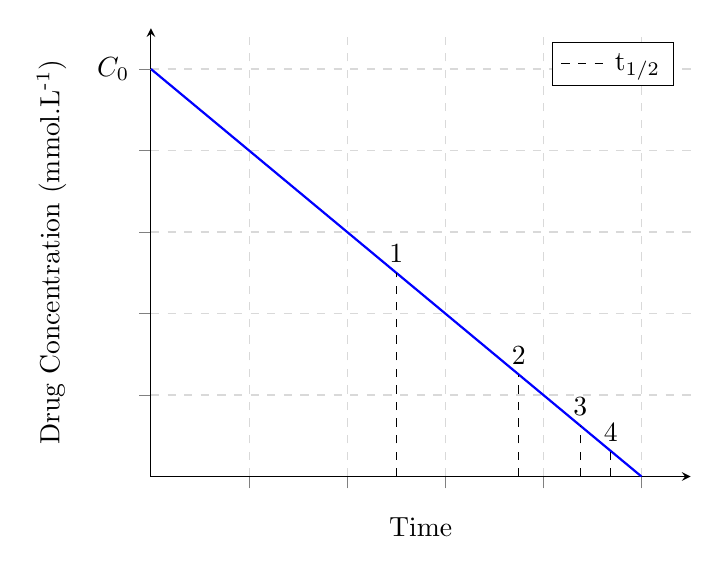
\begin{tikzpicture}

    \begin{axis}[
        axis x line=middle,
        axis y line=middle,
        grid = major,
        grid style={dashed, gray!30},
        xmin=0,     % start the diagram at this x-coordinate
        xmax= 110,    % end   the diagram at this x-coordinate
        ymin= 0,     % start the diagram at this y-coordinate
        ymax= 110,   % end   the diagram at this y-coordinate
        %axis background/.style={fill=white},
    	  x label style={at={(axis description cs:0.5,-0.1)},anchor=north},
	  y label style={at={(axis description cs:-0.1,.5)},rotate=90,anchor=south},
	  xticklabels={},
	 yticklabels={},
	extra y ticks={100},
	extra y tick labels={$C_0$},
	 ylabel near ticks,
	xlabel near ticks,
        xlabel=Time,
        ylabel=Drug Concentration (mmol.L\textsuperscript{-1}),
        tick align=outside,
        enlargelimits=false,
legend pos=north east]

	\addlegendimage{black,thin,dashed};
	\addlegendentry{t\textsubscript{1/2}};

	\addplot[domain=0:100, blue, thick,samples=500] {100-x};

	\draw[black, thin, dashed] (50,0) -- (50,50) node[above]{1};
	\draw[black, thin, dashed] (75,0) -- (75,25) node[above]{2};
	\draw[black, thin, dashed] (87.5,0) -- (87.5,12.5) node[above]{3};
	\draw[black, thin, dashed] (93.75,0) -- (93.75, 6.25) node[above]{4};



	

\end{axis}

\end{tikzpicture} 
\end{document}